\documentclass[aspectratio=169,10pt]{beamer}
\usetheme{Madrid}
\usecolortheme{default}
\usepackage[T1]{fontenc}
\usepackage[utf8]{inputenc}
\usepackage{lmodern}
\usepackage{graphicx}
\usepackage{tikz}
\usetikzlibrary{positioning}
\usepackage{booktabs}
\usepackage{tabularx}
\usepackage{array}
\usepackage{hyperref}
\usepackage{ragged2e}
\usepackage{xcolor}
\graphicspath{{assets/}}

\definecolor{deepblue}{HTML}{163A59}
\definecolor{accent}{HTML}{D97706}
\definecolor{softblue}{HTML}{EAF3FF}
\definecolor{softorange}{HTML}{FFF4E6}
\definecolor{softgreen}{HTML}{EAF8EF}
\definecolor{softpurple}{HTML}{F2ECFA}
\definecolor{dark}{HTML}{111827}
\definecolor{muted}{HTML}{4B5563}

\setbeamercolor{title}{fg=white}
\setbeamercolor{frametitle}{fg=white,bg=deepblue}
\setbeamercolor{structure}{fg=deepblue}
\setbeamercolor{normal text}{fg=dark,bg=white}
\setbeamertemplate{navigation symbols}{}
\setbeamertemplate{footline}[frame number]
\setbeamertemplate{itemize item}{\color{accent}$\blacktriangleright$}
\setbeamertemplate{itemize subitem}{\color{deepblue}$\circ$}

\newcommand{\smallsource}[1]{}
\newcommand{\bigpoint}[1]{\begin{center}\Huge\bfseries\color{deepblue}#1\end{center}}
\newcommand{\twobullets}[2]{\begin{itemize}\item #1\item #2\end{itemize}}
\newcommand{\threebullets}[3]{\begin{itemize}\item #1\item #2\item #3\end{itemize}}
\newcommand{\sectionframe}[2]{
\begin{frame}[plain]
\begin{tikzpicture}[remember picture,overlay]
\node[anchor=center,inner sep=0pt] at (current page.center){\includegraphics[width=\paperwidth,height=\paperheight]{#2}};
\fill[deepblue,opacity=.76] (current page.south west) rectangle (current page.north east);
\node[align=center,text=white,text width=0.90\paperwidth] at (current page.center){\fontsize{24}{30}\selectfont\bfseries #1};
\end{tikzpicture}
\end{frame}}

\newcommand{\imageframe}[4]{
\begin{frame}{#1}
\begin{columns}[T,onlytextwidth]
\column{0.45\textwidth}
\vspace{0.3cm}
#2
\column{0.52\textwidth}
\includegraphics[width=\linewidth,height=0.68\textheight,keepaspectratio]{#3}
\end{columns}
\smallsource{#4}
\end{frame}}

\newcommand{\wideimageframe}[4]{
\begin{frame}{#1}
\begin{center}
\includegraphics[width=#2\linewidth,height=0.66\textheight,keepaspectratio]{#3}
\end{center}
\vspace{-0.1cm}
#4
\end{frame}}

\title{Agentic AI for Economics Research}
\subtitle{Concepts, tools, workflows and responsible use}
\author{Mini-course for PhD students and faculty}
\date{}

\begin{document}

% 1
\begin{frame}[plain]
\begin{tikzpicture}[remember picture,overlay]
\node[anchor=center,inner sep=0pt] at (current page.center){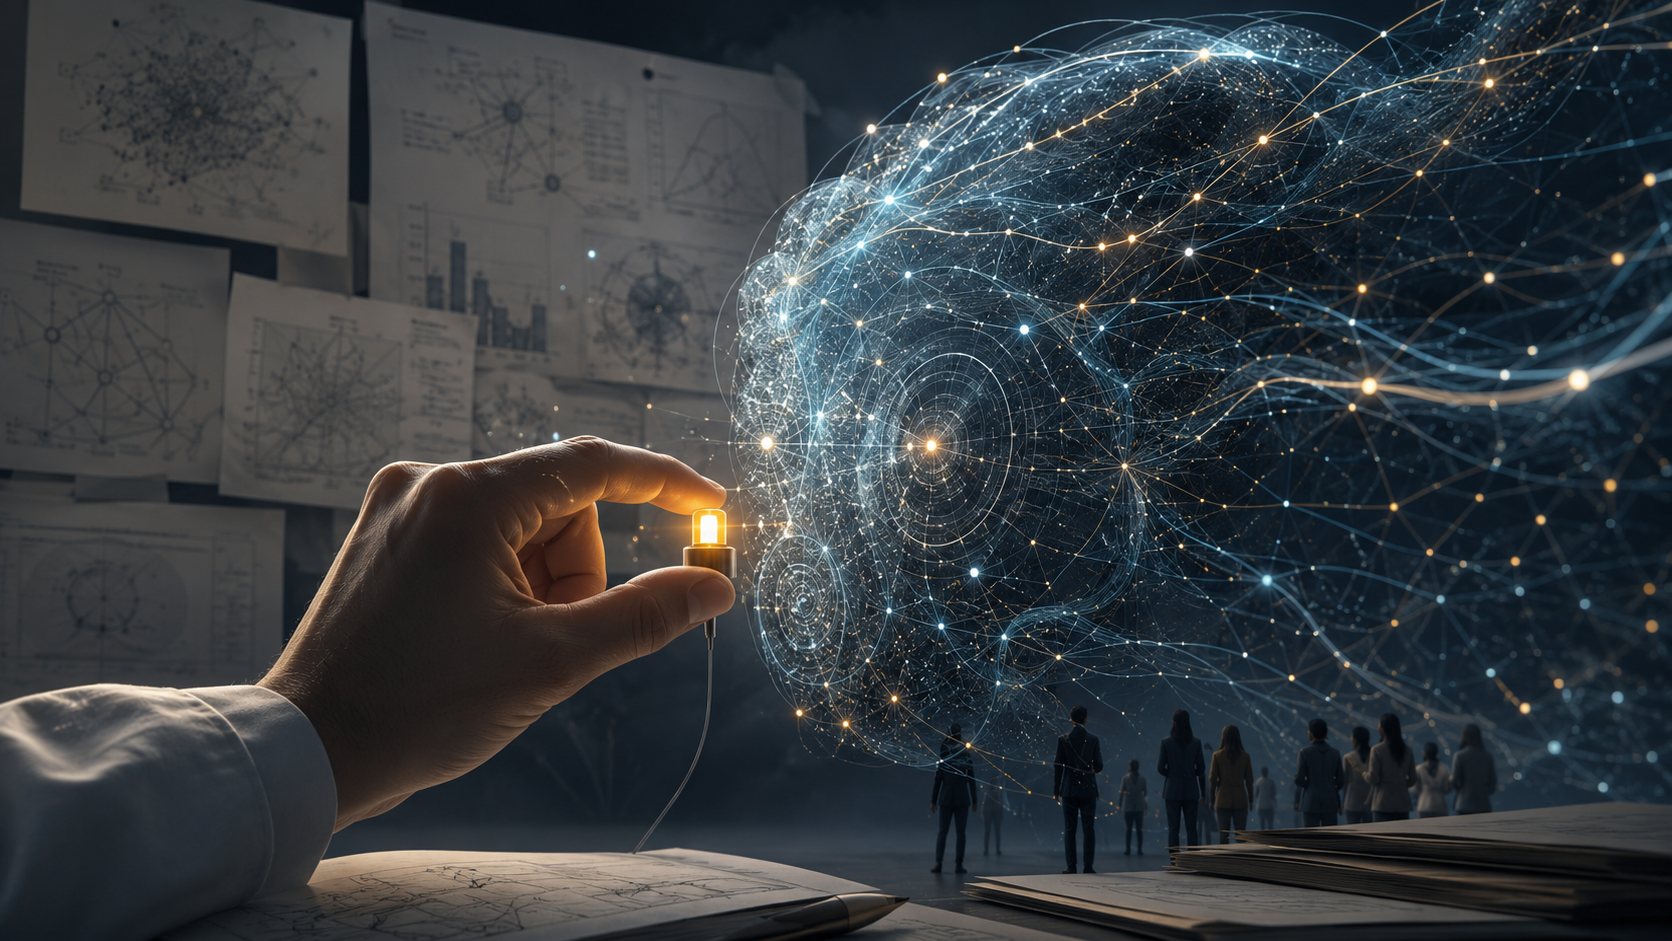
\includegraphics[width=\paperwidth,height=\paperheight]{hero}};
\fill[black,opacity=.45] (current page.south west) rectangle (current page.north east);
\node[align=left,text=white,anchor=west] at ([xshift=0.8cm]current page.west){\fontsize{30}{36}\selectfont\bfseries Agentic AI for\\Economics Research\\[0.3cm]\large Concepts, tools, workflows and responsible use};
\end{tikzpicture}
\end{frame}

% 2
\imageframe{Why this course now?}{\threebullets{AI is moving from \textbf{answering} to \textbf{acting}.}{Research work is full of repeatable tasks: searching, coding, checking, documenting.}{The hard question is no longer ``can it help?'' but \textbf{where should we trust it?}}}{researcher}{Generated editorial illustration.}

% 3
\begin{frame}{Course roadmap}
\begin{center}
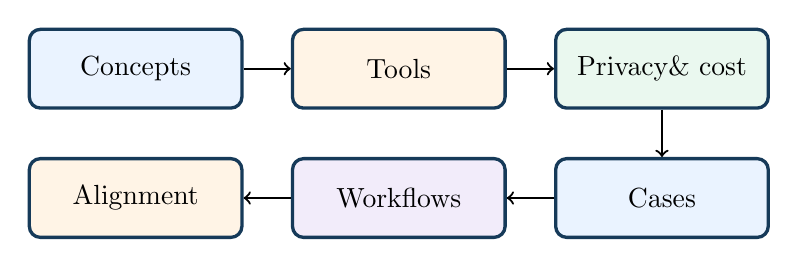
\begin{tikzpicture}[node distance=0.6cm]
\tikzstyle{box}=[rounded corners,draw=deepblue,fill=softblue,very thick,minimum width=2.7cm,minimum height=1cm,align=center]
\node[box] (a) {Concepts};
\node[box,right=of a,fill=softorange] (b) {Tools};
\node[box,right=of b,fill=softgreen] (c) {Privacy\& cost};
\node[box,below=of b,fill=softpurple] (d) {Workflows};
\node[box,right=of d,fill=softblue] (e) {Cases};
\node[box,left=of d,fill=softorange] (f) {Alignment};
\draw[->,thick] (a)--(b); \draw[->,thick] (b)--(c); \draw[->,thick] (c)--(e); \draw[->,thick] (e)--(d); \draw[->,thick] (d)--(f);
\end{tikzpicture}
\end{center}
\vspace{0.4cm}
\bigpoint{A practical map, not a technical manual.}
\end{frame}

\sectionframe{Part 1 - Concepts and vocabulary}{researcher}

% 4
\begin{frame}{What is an AI agent?}
\begin{columns}[T,onlytextwidth]
\column{0.50\textwidth}
\bigpoint{LLM + tools + goal + loop}
\column{0.48\textwidth}
\threebullets{It receives an objective.}{It decides what to inspect or call.}{It iterates until the task looks complete.}
\end{columns}
\vspace{0.5cm}
\begin{center}\large\color{muted}An agent is not just a smarter chatbot. It is a workflow with partial autonomy.\end{center}
\end{frame}

% 5
\begin{frame}{Chatbot vs agent}
\begin{center}
\begin{tabularx}{0.9\linewidth}{>{\bfseries}lXX}
\toprule
 & Chatbot & Agent \\
\midrule
Main action & Responds & Plans and acts \\
Tools & Optional & Central \\
Files & Usually attached & Often browsed and edited \\
Failure mode & Wrong answer & Wrong action \\
Human role & Reader & Supervisor \\
\bottomrule
\end{tabularx}
\end{center}
\end{frame}

% 6
\begin{frame}{The agent loop}
\begin{center}
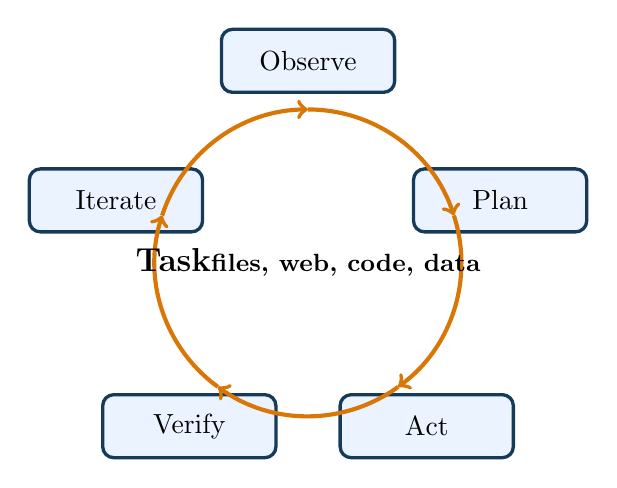
\begin{tikzpicture}[scale=0.95]
\foreach \ang/\txt in {90/Observe,18/Plan,-54/Act,-126/Verify,162/Iterate}{
\node[draw=deepblue,fill=softblue,rounded corners,very thick,minimum width=2.2cm,minimum height=0.8cm] at (\ang:2.7) {\txt};}
\draw[->,line width=1.5pt,color=accent] (90:2.05) arc (90:18:2.05);
\draw[->,line width=1.5pt,color=accent] (18:2.05) arc (18:-54:2.05);
\draw[->,line width=1.5pt,color=accent] (-54:2.05) arc (-54:-126:2.05);
\draw[->,line width=1.5pt,color=accent] (-126:2.05) arc (-126:-198:2.05);
\draw[->,line width=1.5pt,color=accent] (162:2.05) arc (162:90:2.05);
\node[align=center] at (0,0) {\large\bfseries Task\par\small files, web, code, data};
\end{tikzpicture}
\end{center}
\end{frame}

% 7
\begin{frame}{From prompt to task}
\begin{columns}[T,onlytextwidth]
\column{0.46\textwidth}
\textbf{Prompt}\\[0.2cm]
``Explain how to run this regression.''
\column{0.46\textwidth}
\textbf{Task}\\[0.2cm]
``Inspect the scripts, run the model, export the table, check the first stage, and report what changed.''
\end{columns}
\vspace{0.8cm}
\bigpoint{Agentic AI shifts the unit of delegation.}
\end{frame}

% 8
\begin{frame}{Core terminology}
\begin{center}
\begin{tabularx}{0.86\linewidth}{>{\bfseries}lX}
\toprule
Context & What the model can see right now. \\
Tool & Something the model can call: browser, shell, files, database. \\
Memory & Persistent information across sessions or projects. \\
Sandbox & A controlled environment where actions are constrained. \\
Permission & The boundary between suggestion and action. \\
\bottomrule
\end{tabularx}
\end{center}
\end{frame}

% 9
\wideimageframe{Context and token load}{0.86}{token_clean}{\begin{center}\large Context, tool calls and verification are why agents feel expensive.\end{center}}

% 10
\begin{frame}{Subscription vs API}
\begin{columns}[T,onlytextwidth]
\column{0.48\textwidth}
\textbf{Subscription}\\[0.2cm]
\twobullets{Simple monthly price.}{Limits are often soft, dynamic or hard to compare.}
\column{0.48\textwidth}
\textbf{API / metered usage}\\[0.2cm]
\twobullets{Cost is measurable per token or call.}{Easier to budget, but easier to overspend.}
\end{columns}
\vspace{0.5cm}
\begin{center}\Large\color{accent}\bfseries For agents, ``unlimited'' rarely means uncontrolled.\end{center}
\smallsource{Pricing pages change frequently; update examples before teaching.}
\end{frame}

\sectionframe{Part 2 - Tools and interfaces}{hero}

% 12
\wideimageframe{Four main environments}{0.90}{tools_clean}{\begin{center}\large The point is not to memorize tools, but to choose the right environment for the task.\end{center}}

% 13
\begin{frame}{1. Chat / app environments}
\begin{columns}[T,onlytextwidth]
\column{0.52\textwidth}
\threebullets{ChatGPT, Claude, Gemini, Grok and similar apps.}{Best for thinking, writing, summarizing and light analysis.}{Weak point: file control, reproducibility and hidden limits.}
\column{0.44\textwidth}
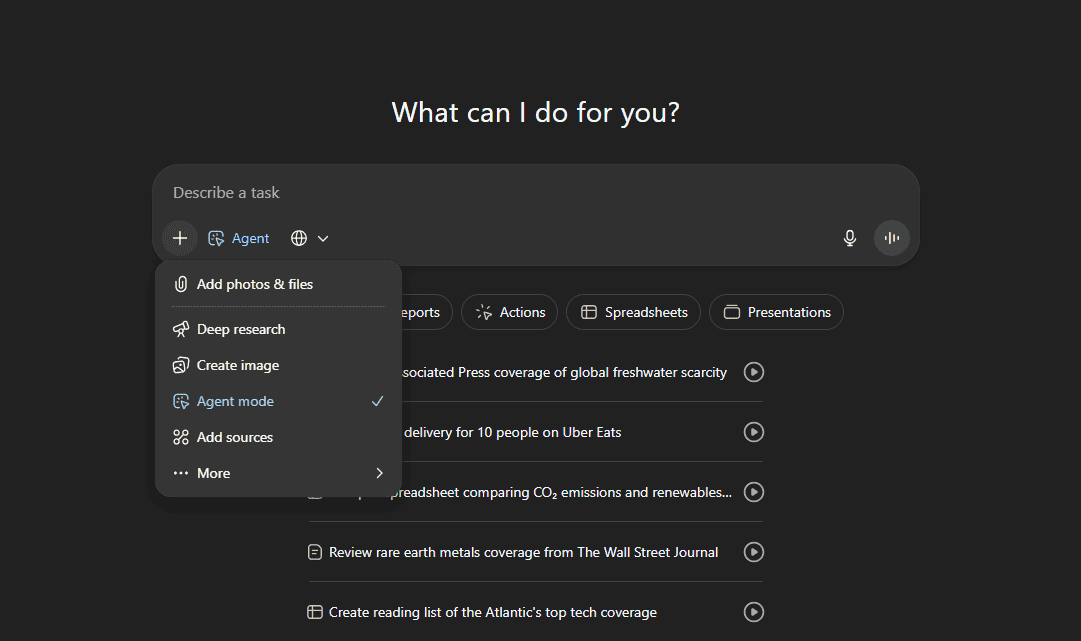
\includegraphics[width=\linewidth,height=.65\textheight,keepaspectratio]{chatgpt}
\end{columns}
\smallsource{Screenshot from BKA Content article on ChatGPT Agent Mode.}
\end{frame}

% 14
\begin{frame}{2. Research and browser assistants}
\begin{columns}[T,onlytextwidth]
\column{0.48\textwidth}
\textbf{Examples}\\[0.2cm]
Perplexity-style search, Elicit, NotebookLM, Deep Research, browser agents, and AI search tools.
\column{0.48\textwidth}
\textbf{Use}\\[0.2cm]
Source discovery, evidence extraction, paper triage, background memos.
\end{columns}
\vspace{0.7cm}
\begin{center}\Large\bfseries\color{deepblue}Good for finding; not enough for believing.\end{center}
\end{frame}

% 15
\begin{frame}{3. IDE agents}
\begin{columns}[T,onlytextwidth]
\column{0.48\textwidth}
\threebullets{Cursor, VS Code/Copilot, Codex-style coding environments.}{Best when the object is a codebase.}{Review happens through diffs, tests and file changes.}
\column{0.48\textwidth}
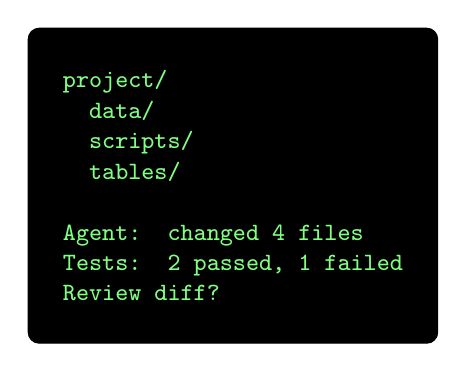
\begin{tikzpicture}
\node[draw,rounded corners,fill=black,text=green!50!white,minimum width=5.2cm,minimum height=4cm,align=left,font=\ttfamily\small] {project/\\\quad data/\\\quad scripts/\\\quad tables/\\\\ Agent: changed 4 files\\ Tests: 2 passed, 1 failed\\ Review diff?};
\end{tikzpicture}
\end{columns}
\end{frame}

% 16
\begin{frame}{4. CLI and local agents}
\begin{columns}[T,onlytextwidth]
\column{0.47\textwidth}
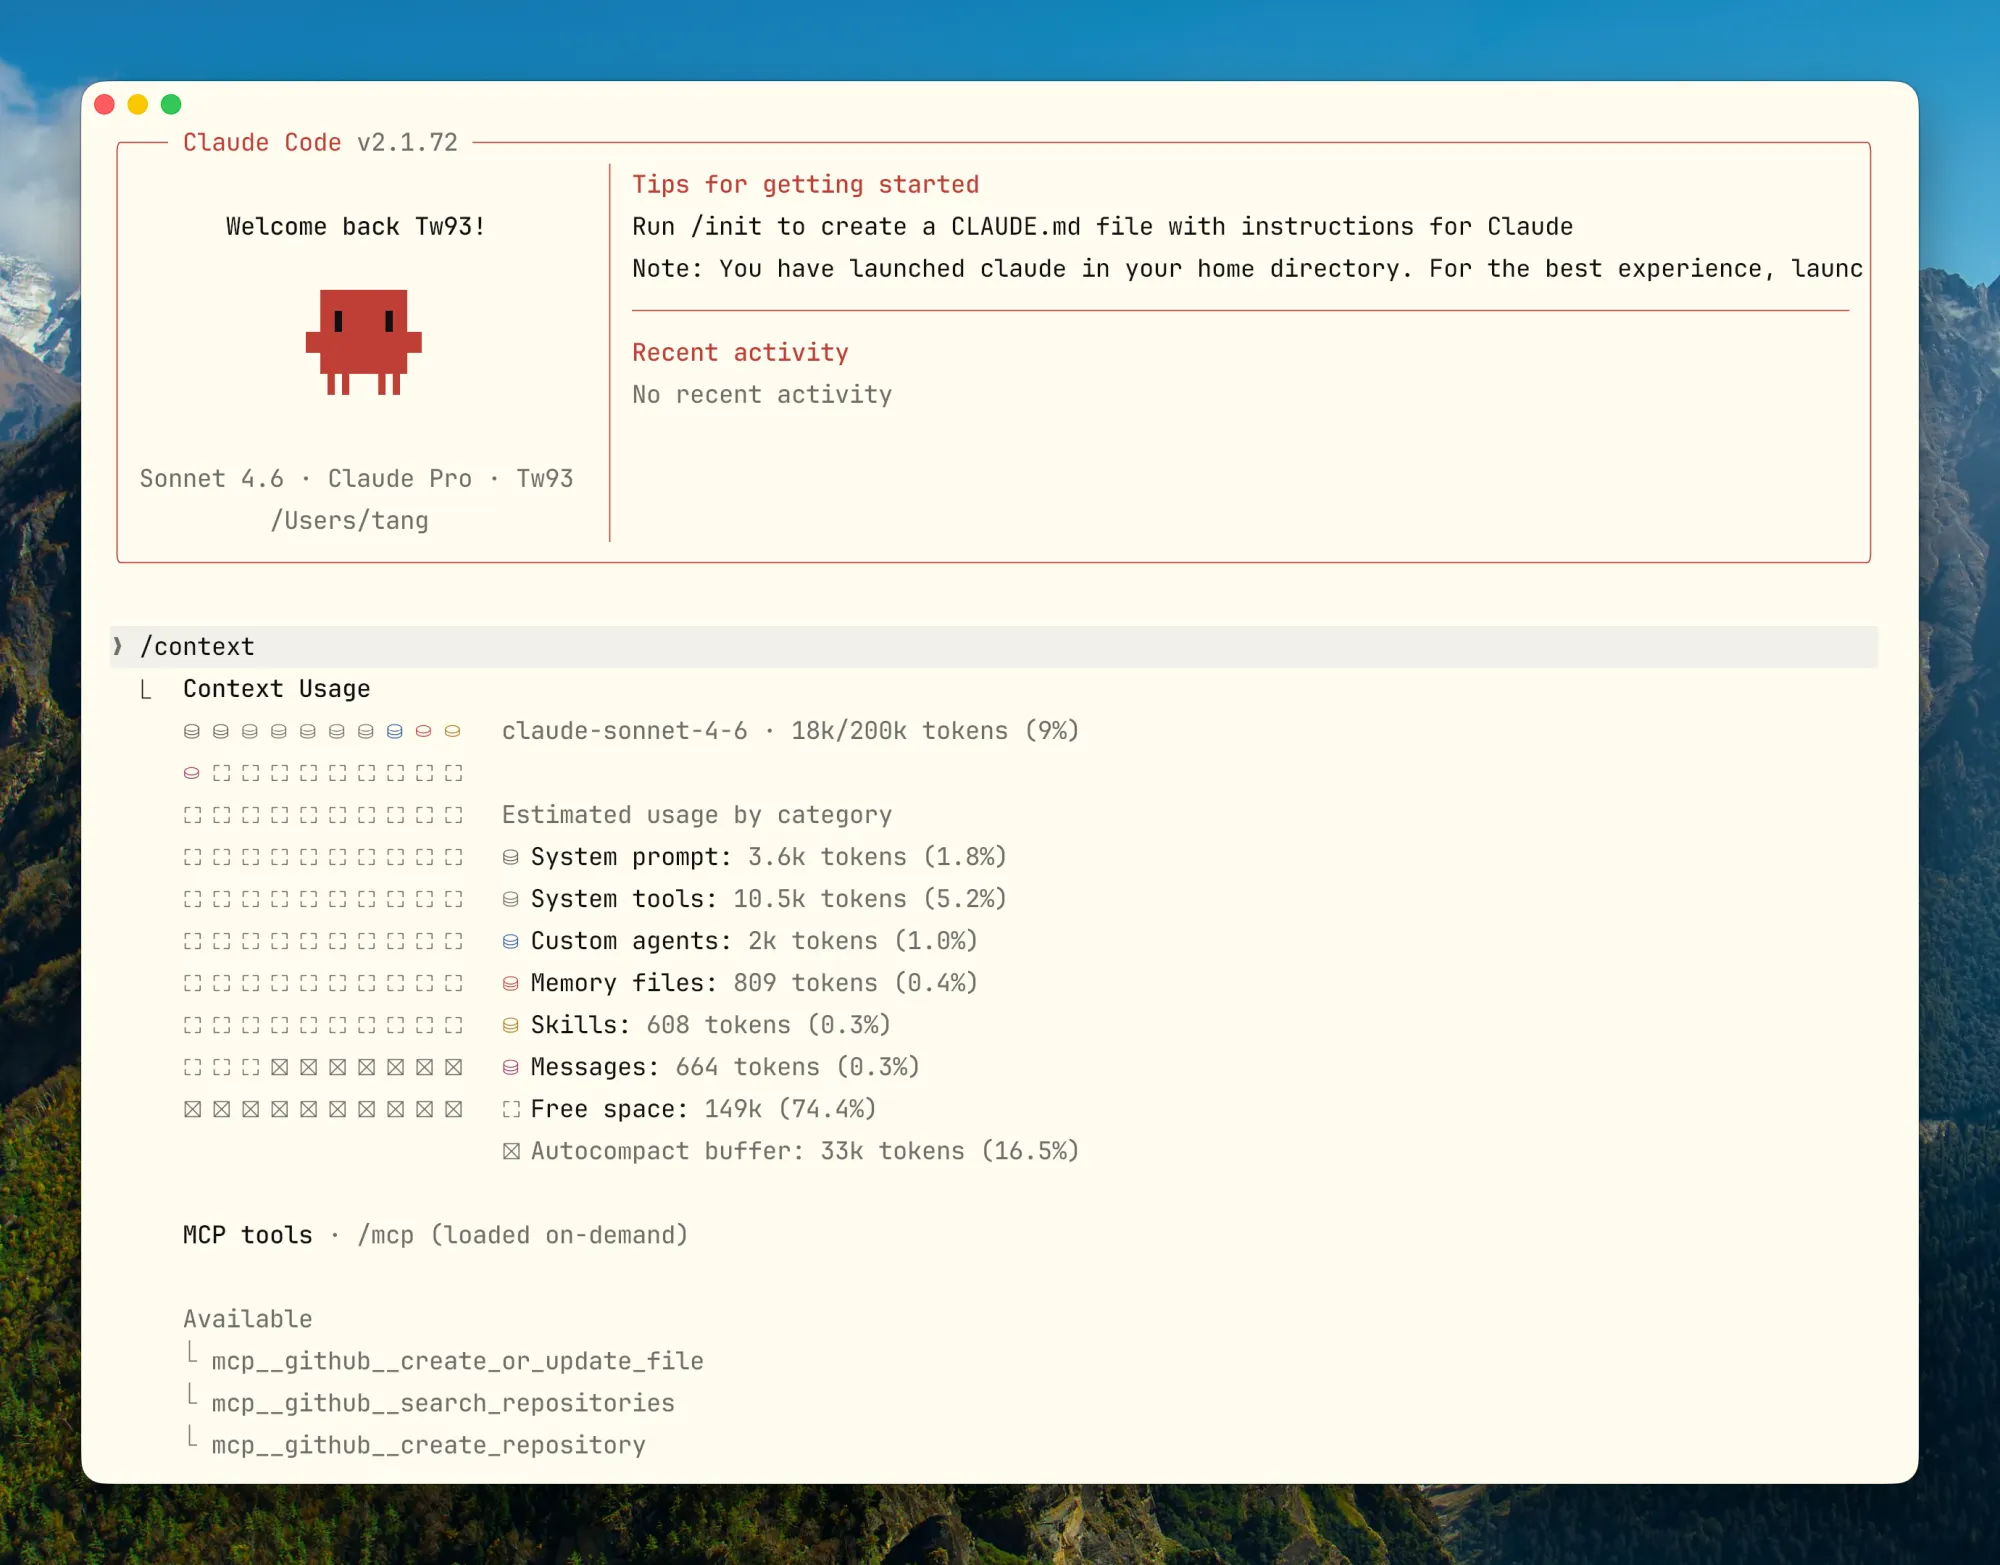
\includegraphics[width=\linewidth,height=.68\textheight,keepaspectratio]{claude}
\column{0.50\textwidth}
\threebullets{Claude Code, Gemini CLI, Aider, Codex CLI, Ollama/LM Studio workflows, plus local Llama, Qwen or Mistral models.}{Powerful because they can inspect folders and run commands.}{Riskier because mistakes can change files or execute code.}
\end{columns}
\smallsource{Claude Code terminal screenshot from Tw93 article.}
\end{frame}

% 18

\begin{frame}{Comparing the main ecosystems, without religion}
\begin{center}
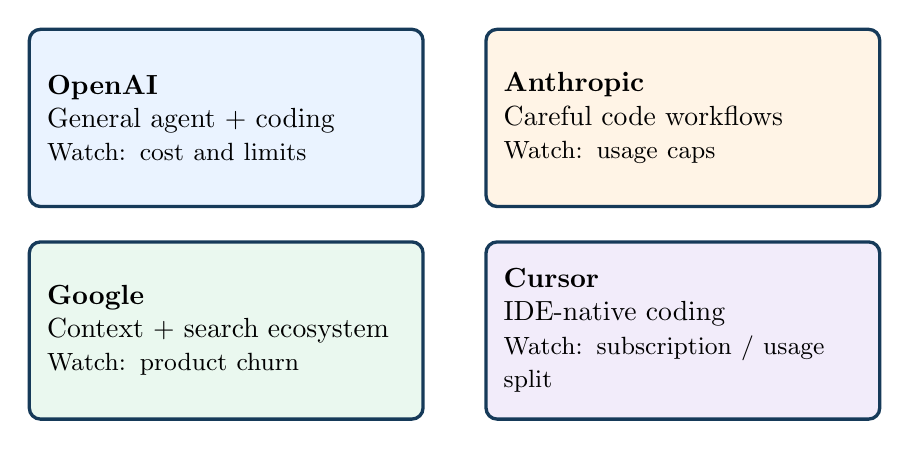
\begin{tikzpicture}[node distance=.45cm]
\tikzstyle{card}=[rounded corners,draw=deepblue,very thick,minimum width=5.0cm,minimum height=2.25cm,align=left,text width=4.55cm]
\node[card,fill=softblue] (openai) at (0,1.5) {\textbf{OpenAI}\\General agent + coding\\\small Watch: cost and limits};
\node[card,fill=softorange] (anthropic) at (5.8,1.5) {\textbf{Anthropic}\\Careful code workflows\\\small Watch: usage caps};
\node[card,fill=softgreen] (google) at (0,-1.2) {\textbf{Google}\\Context + search ecosystem\\\small Watch: product churn};
\node[card,fill=softpurple] (cursor) at (5.8,-1.2) {\textbf{Cursor}\\IDE-native coding\\\small Watch: subscription / usage split};
\end{tikzpicture}
\end{center}
\vspace{0.1cm}
\begin{center}\small Other scenarios: Grok/X for app use; Perplexity/Elicit/NotebookLM for search; Llama/Qwen/Mistral for local experiments.\end{center}
\end{frame}

% 19
\begin{frame}{Pricing snapshot: how to teach it}
\begin{columns}[T,onlytextwidth]
\column{0.48\textwidth}
\textbf{Do not teach a frozen price table.}\\[0.2cm]
\twobullets{Plans change faster than syllabi.}{Explain the cost logic instead.}
\column{0.48\textwidth}
\textbf{Teach three questions.}\\[0.2cm]
\threebullets{Is usage capped or metered?}{Is agent usage separate?}{Are business data protected?}
\end{columns}
\smallsource{OpenAI, Anthropic, Google and Cursor pricing pages consulted.}
\end{frame}

% 21
\begin{frame}{App vs CLI vs IDE}
\begin{center}
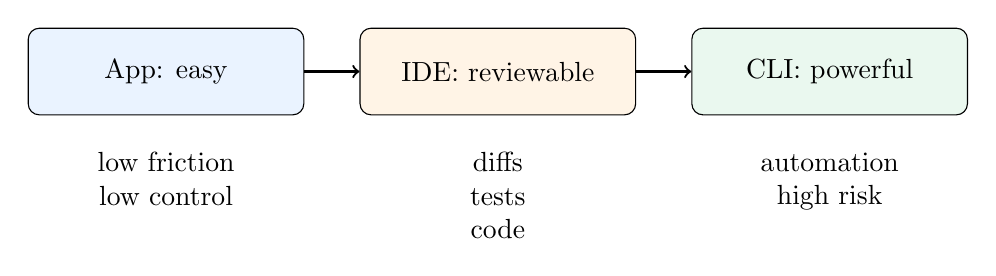
\begin{tikzpicture}[node distance=.7cm]
\node[draw,rounded corners,fill=softblue,minimum width=3.5cm,minimum height=1.1cm] (app) {App: easy};
\node[draw,rounded corners,fill=softorange,minimum width=3.5cm,minimum height=1.1cm,right=of app] (ide) {IDE: reviewable};
\node[draw,rounded corners,fill=softgreen,minimum width=3.5cm,minimum height=1.1cm,right=of ide] (cli) {CLI: powerful};
\draw[->,thick] (app)--(ide); \draw[->,thick] (ide)--(cli);
\node[below=.35cm of app,align=center] {low friction\\ low control};
\node[below=.35cm of ide,align=center] {diffs\\ tests\\ code};
\node[below=.35cm of cli,align=center] {automation\\ high risk};
\end{tikzpicture}
\end{center}
\vspace{0.5cm}
\bigpoint{Choose the interface by task, not by brand.}
\end{frame}

\sectionframe{Part 3 - Execution environments}{team}

% 23
\begin{frame}{Folder access: the real boundary}
\begin{center}
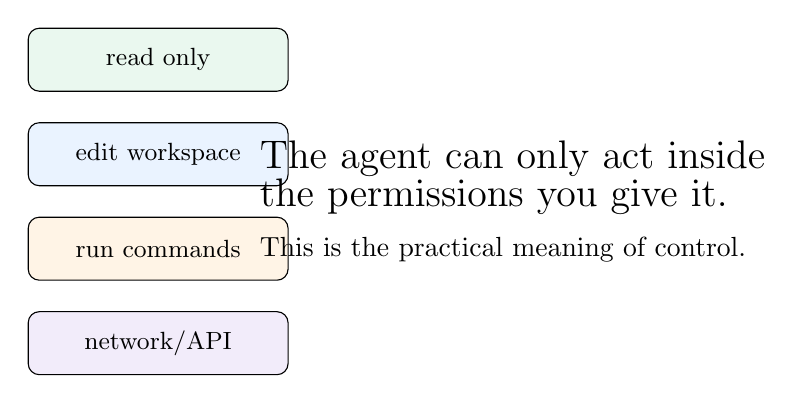
\begin{tikzpicture}[font=\small]
\node[draw,rounded corners,fill=softgreen,minimum width=3.3cm,minimum height=.8cm] at (0,2) {read only};
\node[draw,rounded corners,fill=softblue,minimum width=3.3cm,minimum height=.8cm] at (0,.8) {edit workspace};
\node[draw,rounded corners,fill=softorange,minimum width=3.3cm,minimum height=.8cm] at (0,-.4) {run commands};
\node[draw,rounded corners,fill=softpurple,minimum width=3.3cm,minimum height=.8cm] at (0,-1.6) {network/API};
\node[align=left] at (4.5,.2) {\Large The agent can only act inside\\\Large the permissions you give it.\\[0.25cm]\normalsize This is the practical meaning of control.};
\end{tikzpicture}
\end{center}
\end{frame}

% 24
\begin{frame}{Sandbox}
\begin{columns}[T,onlytextwidth]
\column{0.48\textwidth}
\bigpoint{A safe place to be wrong}
\column{0.48\textwidth}
\threebullets{Run code away from your main machine.}{Limit file, network and system access.}{Make destructive actions reversible.}
\end{columns}
\end{frame}

\sectionframe{Part 4 - Privacy, cost and governance}{hero}

% 27
\begin{frame}{Does it train on my data?}
\begin{columns}[T,onlytextwidth]
\column{0.48\textwidth}
\textbf{The honest answer:}\\[0.2cm]
It depends on the provider, plan, workspace and settings.
\column{0.48\textwidth}
\textbf{What to check:}\\[0.2cm]
\threebullets{consumer vs business plan;}{API vs app usage;}{retention and training settings.}
\end{columns}
\smallsource{OpenAI Business page notes no training on business data by default; always verify provider-specific settings.}
\end{frame}

% 28
\begin{frame}{Data risk in economics research}
\begin{center}
\begin{tabularx}{0.9\linewidth}{>{\bfseries}lX}
\toprule
High risk & microdata, administrative data, embargoed data, confidential referee reports \\
Medium risk & unpublished drafts, grant ideas, collaborator data \\
Lower risk & public documentation, synthetic examples, teaching material \\
\bottomrule
\end{tabularx}
\end{center}
\vspace{0.4cm}
\begin{center}\Large\bfseries\color{accent}When in doubt: anonymize, abstract, or use a sandbox.\end{center}
\end{frame}

% 29
\begin{frame}{Extra usage and cost spikes}
\begin{columns}[T,onlytextwidth]
\column{0.48\textwidth}
\threebullets{Agents read more context.}{They call tools repeatedly.}{They may retry after errors.}
\column{0.48\textwidth}
\textbf{Practical safeguards}\\[0.2cm]
\threebullets{Set a budget.}{Ask for a plan before execution.}{Use cheaper models for scanning.}
\end{columns}
\end{frame}

% 31
\begin{frame}{Hallucinations are not only fake citations}
\begin{center}
\begin{tabularx}{0.86\linewidth}{>{\bfseries}lX}
\toprule
Citation & plausible but nonexistent source \\
Code & function that runs but implements the wrong logic \\
Statistics & correct syntax, wrong interpretation \\
Workflow & task marked complete without real verification \\
\bottomrule
\end{tabularx}
\end{center}
\end{frame}

% 32
\wideimageframe{Control strategies}{0.72}{funnel}{\begin{center}\large Agentic work is safest when verification is designed into the workflow.\end{center}}

\sectionframe{Part 5 - Agentic architecture}{team}

% 34
\begin{frame}{Rules and Markdown files}
\begin{columns}[T,onlytextwidth]
\column{0.45\textwidth}
\bigpoint{Rules are prompts that stay.}
\column{0.5\textwidth}
\threebullets{Project style and conventions.}{What the agent must not do.}{How to test before saying done.}
\end{columns}
\vspace{0.3cm}
\begin{center}\texttt{AGENTS.md} \quad \texttt{CLAUDE.md} \quad \texttt{GEMINI.md} \quad project instructions\end{center}
\end{frame}

% 36
\begin{frame}{RAG in one slide}
\begin{columns}[T,onlytextwidth]
\column{0.45\textwidth}
\bigpoint{Retrieve before generating}
\column{0.50\textwidth}
\twobullets{Instead of stuffing everything into context, retrieve the relevant fragments.}{For research, RAG is often about traceability more than automation.}
\end{columns}
\end{frame}

% 37
\begin{frame}{MCP vs API vs CLI}
\begin{center}
\begin{tabularx}{0.9\linewidth}{>{\bfseries}lX}
\toprule
API & a programmatic endpoint: your code calls a service \\
CLI & a command-line tool: the agent or human runs commands \\
MCP & a standard way to expose tools and data sources to agents \\
\bottomrule
\end{tabularx}
\end{center}
\vspace{0.3cm}
\begin{center}\Large\bfseries\color{accent}MCP is plumbing; CLI is operation; API is integration.\end{center}
\end{frame}

% 38
\begin{frame}{Subagents}
\begin{columns}[T,onlytextwidth]
\column{0.45\textwidth}
\threebullets{Specialized workers for separate tasks.}{Useful for independent review.}{Dangerous when they amplify each other's errors.}
\column{0.52\textwidth}
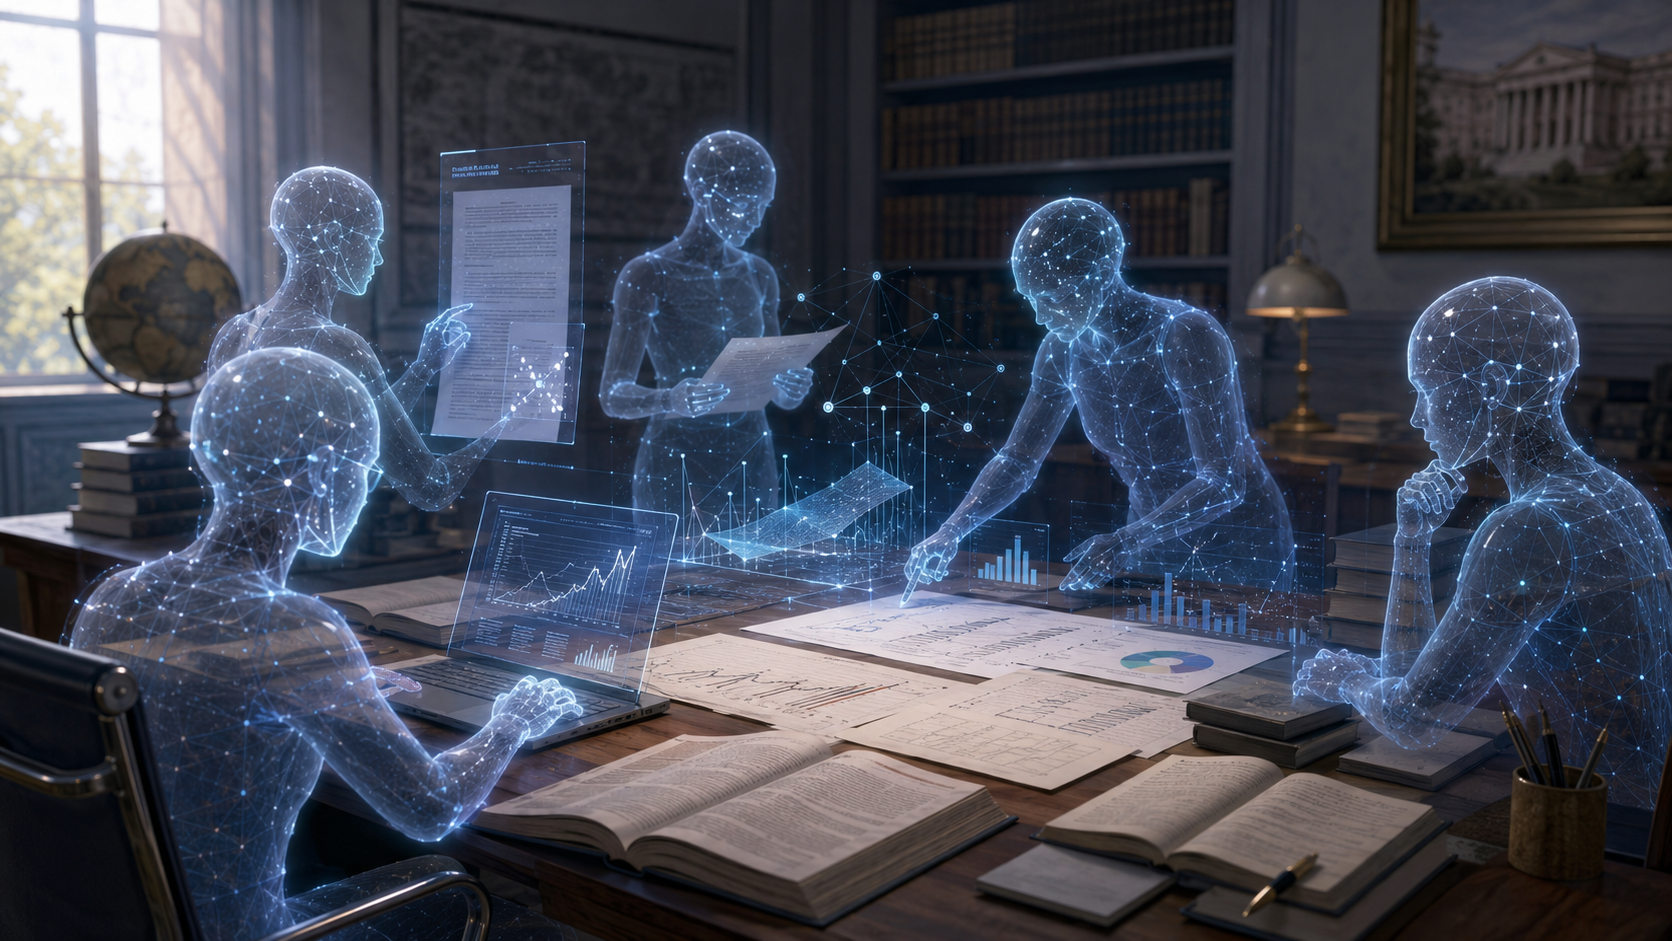
\includegraphics[width=\linewidth,height=.65\textheight,keepaspectratio]{team}
\end{columns}
\smallsource{Generated illustration of collaborative AI assistants.}
\end{frame}

% 39
\begin{frame}{Skills, hooks and loops}
\begin{columns}[T,onlytextwidth]
\column{0.48\textwidth}
\textbf{Skills}\\[0.2cm]
Reusable procedures: ``how we make a figure'', ``how we check tables''.
\column{0.48\textwidth}
\textbf{Hooks / loops}\\[0.2cm]
Automatic checks before or after an agent acts.
\end{columns}
\vspace{0.5cm}
\begin{center}\large Best use: turn tacit lab habits into explicit workflows.\end{center}
\end{frame}

% 40
\begin{frame}{Team of agents and parallelization}
\begin{columns}[T,onlytextwidth]
\column{0.48\textwidth}
\threebullets{Parallelize independent, verifiable tasks.}{Use one orchestrator: human, main agent, or task board.}{Compare disagreements, not just outputs.}
\column{0.48\textwidth}
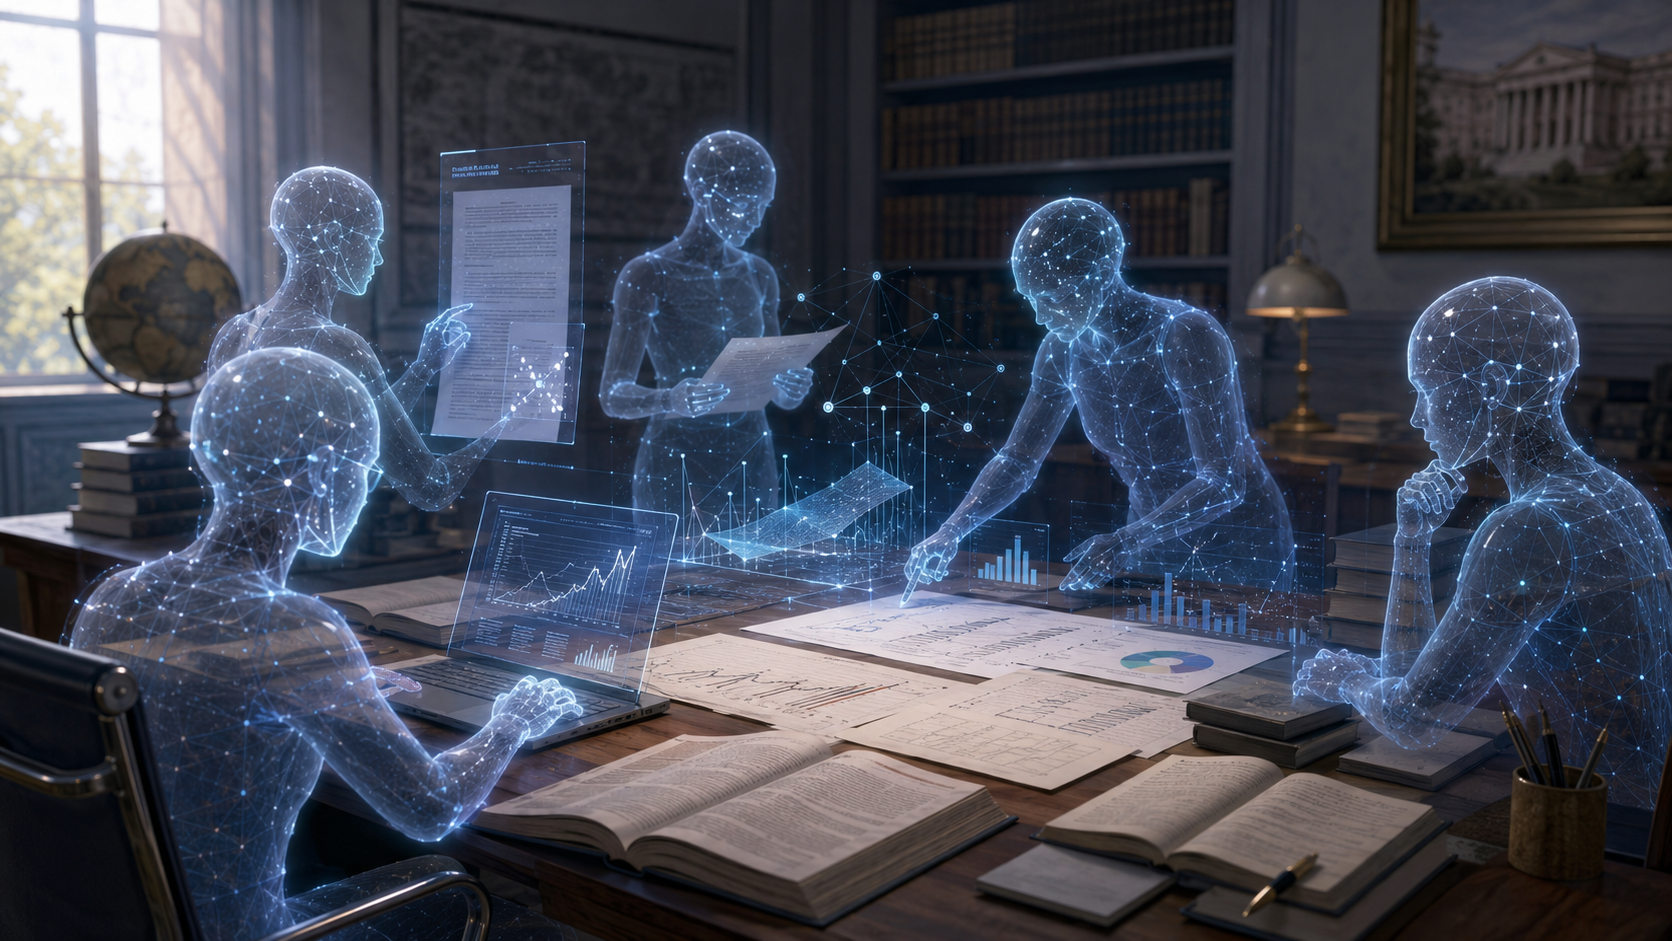
\includegraphics[width=\linewidth,height=.6\textheight,keepaspectratio]{team}
\end{columns}
\end{frame}

\sectionframe{Part 6 - Economics research workflows}{workflow}

% 42
\begin{frame}{Typical agentic workflow}
\begin{center}
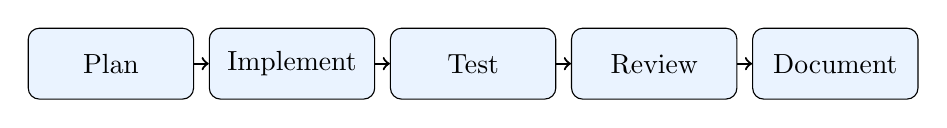
\begin{tikzpicture}[node distance=.5cm]
\foreach \i/\txt in {0/Plan,1/Implement,2/Test,3/Review,4/Document}{
\node[draw,rounded corners,fill=softblue,minimum width=2.1cm,minimum height=.9cm] (n\i) at (\i*2.3,0) {\txt};
\ifnum\i>0 \draw[->,thick] (n\the\numexpr\i-1\relax)--(n\i); \fi}
\end{tikzpicture}
\end{center}
\vspace{0.5cm}
\begin{center}\large Good prompts ask the agent to move through these phases explicitly.\end{center}
\end{frame}

% 43
\begin{frame}{What humans should keep}
\begin{center}
\begin{tabularx}{0.9\linewidth}{>{\bfseries}lX}
\toprule
Theory & what is the mechanism? \\
Identification & what variation identifies the effect? \\
Measurement & what does the variable really capture? \\
Interpretation & what can and cannot be claimed? \\
Responsibility & who signs the paper? \\
\bottomrule
\end{tabularx}
\end{center}
\end{frame}

% 44
\wideimageframe{Economics workflow map}{0.94}{workflow}{\begin{center}\large Agents are useful across the pipeline, but not equally trustworthy at every stage.\end{center}}

% 45
\begin{frame}{Case 1 - Literature review}
\begin{columns}[T,onlytextwidth]
\column{0.48\textwidth}
\textbf{Agent helps with}\\[0.2cm]
\threebullets{search strings and inclusion rules;}{paper summaries and comparison tables;}{citation checking.}
\column{0.48\textwidth}
\textbf{Human keeps}\\[0.2cm]
\twobullets{what counts as relevant;}{how the literature changes the research design.}
\end{columns}
\end{frame}

% 46
\begin{frame}{Case 2 - Data documentation}
\begin{center}\Large\bfseries\color{deepblue}The agent can turn messy data work into explicit documentation.\end{center}
\vspace{0.5cm}
\threebullets{Create a codebook from scripts and raw variable names.}{Detect undocumented transformations.}{Write a replication README.}
\end{frame}

% 47
\begin{frame}{Case 3 - Stata/R/Python debugging}
\begin{columns}[T,onlytextwidth]
\column{0.5\textwidth}
\textbf{Good agent task}\\[0.2cm]
``Find the minimal failing example and propose a patch.''
\column{0.45\textwidth}
\textbf{Bad agent task}\\[0.2cm]
``Fix my project.''
\end{columns}
\vspace{0.7cm}
\bigpoint{Narrow the problem before giving autonomy.}
\end{frame}

% 48
\begin{frame}{Case 4 - Econometric tables and robustness}
\begin{columns}[T,onlytextwidth]
\column{0.48\textwidth}
\threebullets{Generate table-export code.}{Check specification consistency.}{Report which coefficients moved.}
\column{0.48\textwidth}
\threebullets{Do not let the agent pick the preferred result.}{Do not outsource identification.}{Always inspect logs and sample changes.}
\end{columns}
\end{frame}

% 50
\begin{frame}{Case 5 - Referee reports, grants, teaching}
\begin{center}
\begin{tabularx}{0.9\linewidth}{>{\bfseries}lX}
\toprule
Referee report & organize comments, draft tone, check internal consistency \\
Grant proposal & work packages, risks, timeline, non-technical summary \\
Teaching & slides, exercises, rubrics, examples, translations \\
\bottomrule
\end{tabularx}
\end{center}
\end{frame}

\sectionframe{Part 7 - Mobile and daily research practice}{mobile}

% 53
\imageframe{Mobile as control plane}{\threebullets{The phone is not ideal for deep code review.}{It is excellent for orchestration, notes and quick checks.}{Voice prompts can become issues, TODOs or research diary entries.}}{mobile}{Generated illustration of mobile agent orchestration.}

\sectionframe{Part 8 - Alignment, responsibility and conclusion}{hero}

% 55
\begin{frame}{Alignment starts small}
\begin{center}\Large\bfseries\color{deepblue}The local alignment problem:\end{center}
\vspace{0.3cm}
\begin{center}\Large The agent optimizes for completing the task, but you care about doing good research.\end{center}
\vspace{0.5cm}
\threebullets{Plausible code is not valid code.}{A complete table is not a correct table.}{A polished paragraph is not a justified claim.}
\end{frame}

% 57
\begin{frame}{A provocative closing text}
\begin{center}\Large\bfseries\emph{If Anyone Builds It, Everyone Dies}\end{center}
\vspace{0.4cm}
\twobullets{Yudkowsky and Soares offer one of the strongest pessimistic formulations of advanced AI risk.}{Whether or not one accepts the conclusion, it is useful for asking: what happens when autonomy exceeds control?}
\vspace{0.4cm}
\begin{center}\large For this course, the practical lesson is modest: \textbf{never delegate without a control structure}.\end{center}
\smallsource{Eliezer Yudkowsky and Nate Soares, 2025.}
\end{frame}

% 58
\begin{frame}{Final take-home messages}
\begin{center}
\begin{tabularx}{0.9\linewidth}{>{\bfseries}lX}
\toprule
1 & Agents are workflows, not magic assistants. \\
2 & The right interface depends on the task. \\
3 & Privacy, cost and reproducibility are design choices. \\
4 & The best human role is supervisor, theorist and final judge. \\
5 & Alignment is not only a future problem; it is a daily research problem. \\
\bottomrule
\end{tabularx}
\end{center}
\end{frame}

% 60
\begin{frame}{Sources and update checklist}
\scriptsize
\begin{itemize}
\item OpenAI ChatGPT pricing and Business data controls: \url{https://chatgpt.com/pricing/}, \url{https://openai.com/business/chatgpt-pricing/}
\item Anthropic Claude pricing and Claude Code limits: \url{https://claude.com/pricing}, \url{https://www.anthropic.com/news/higher-limits-spacex}
\item Google AI plans: \url{https://one.google.com/intl/en/about/google-ai-plans/}
\item Cursor pricing and product overview: \url{https://cursor.com/pricing}, \url{https://cursor.com/}
\item Screenshots and illustrations used for teaching purposes; replace with institutional screenshots or live demos if preferred.\item Examples mentioned across the deck: ChatGPT, Claude, Gemini, Grok, Perplexity, Elicit, NotebookLM, Cursor, Copilot, Claude Code, Gemini CLI, Codex CLI, Aider, Ollama, LM Studio, Llama, Qwen, Mistral.
\item Before teaching, update: prices, plan names, training/privacy defaults, availability of agent features, and institutional rules.
\end{itemize}
\vfill
\begin{center}\Large\bfseries\color{deepblue}End\end{center}
\end{frame}

\end{document}
